\begin{frame}
  \frametitle{Geometry of \gls{MSBR} model for SERPENT 2}
    \vspace{-0.2in}
      \begin{figure}[t]
    \hspace*{-0.35in}
        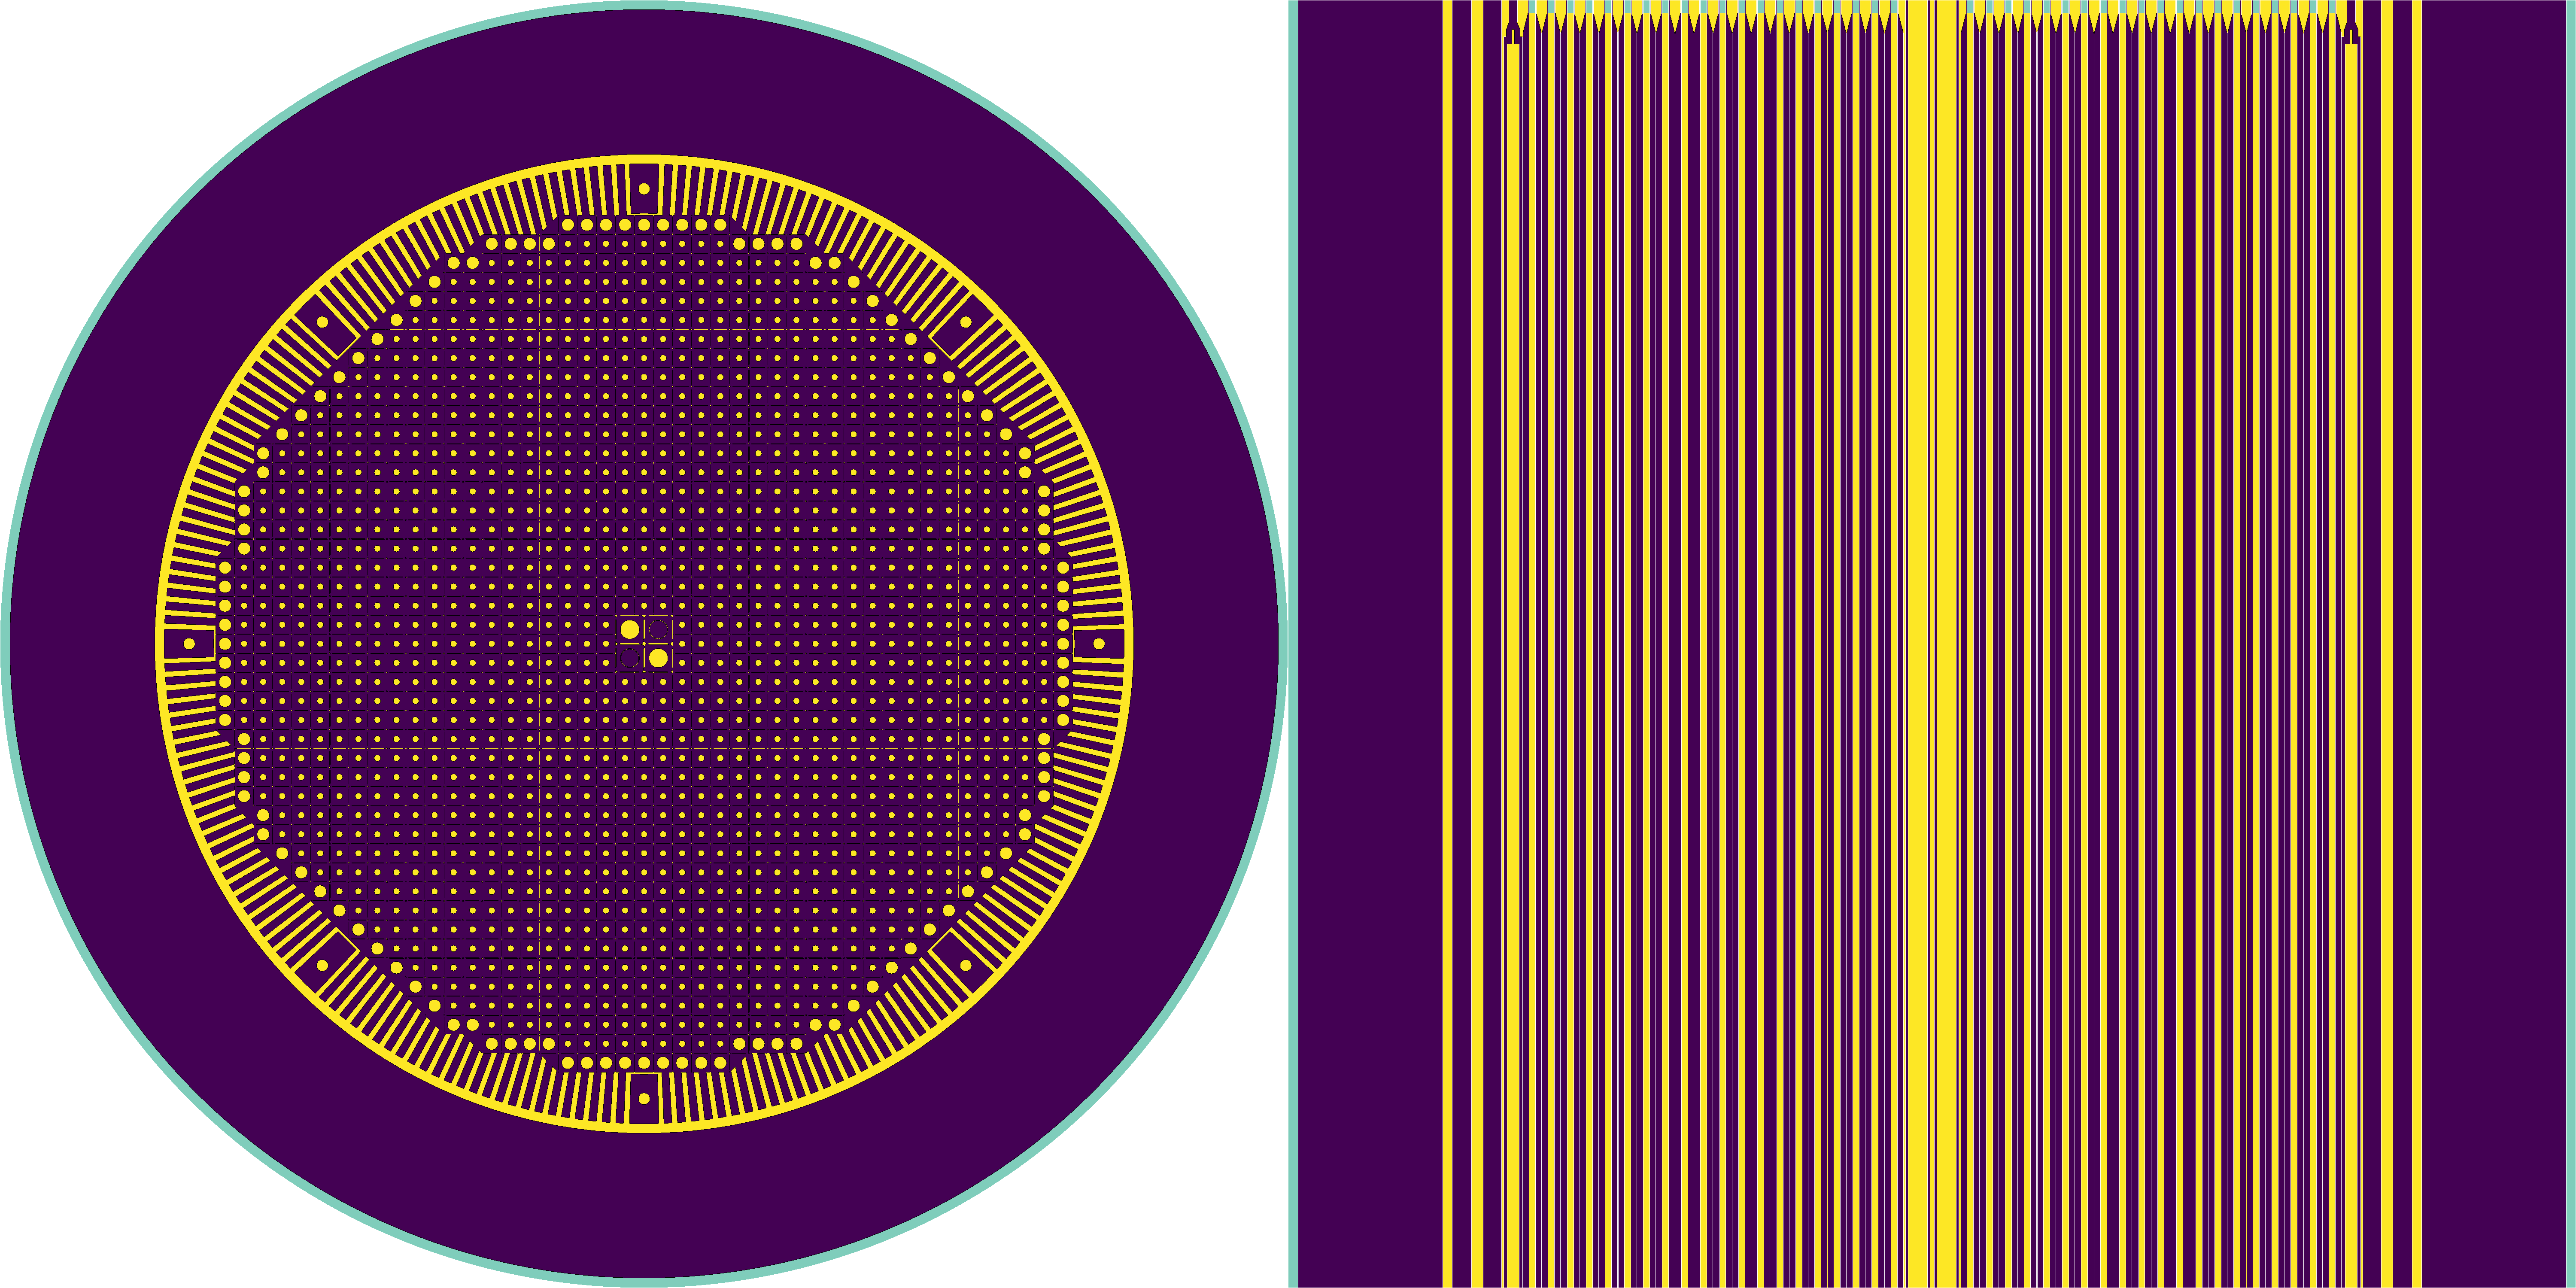
\includegraphics[height=0.75\textheight]{./images/geometry_main_views.png}
        \caption{Plan (left) and elevation (right) view of \gls{MSBR} model}
  \end{figure}


\end{frame}

\begin{frame}
  \frametitle{Graphite elements geometry}
  \begin{figure}[t]
     \vspace{-0.20in}
       \hspace*{-0.4in}
       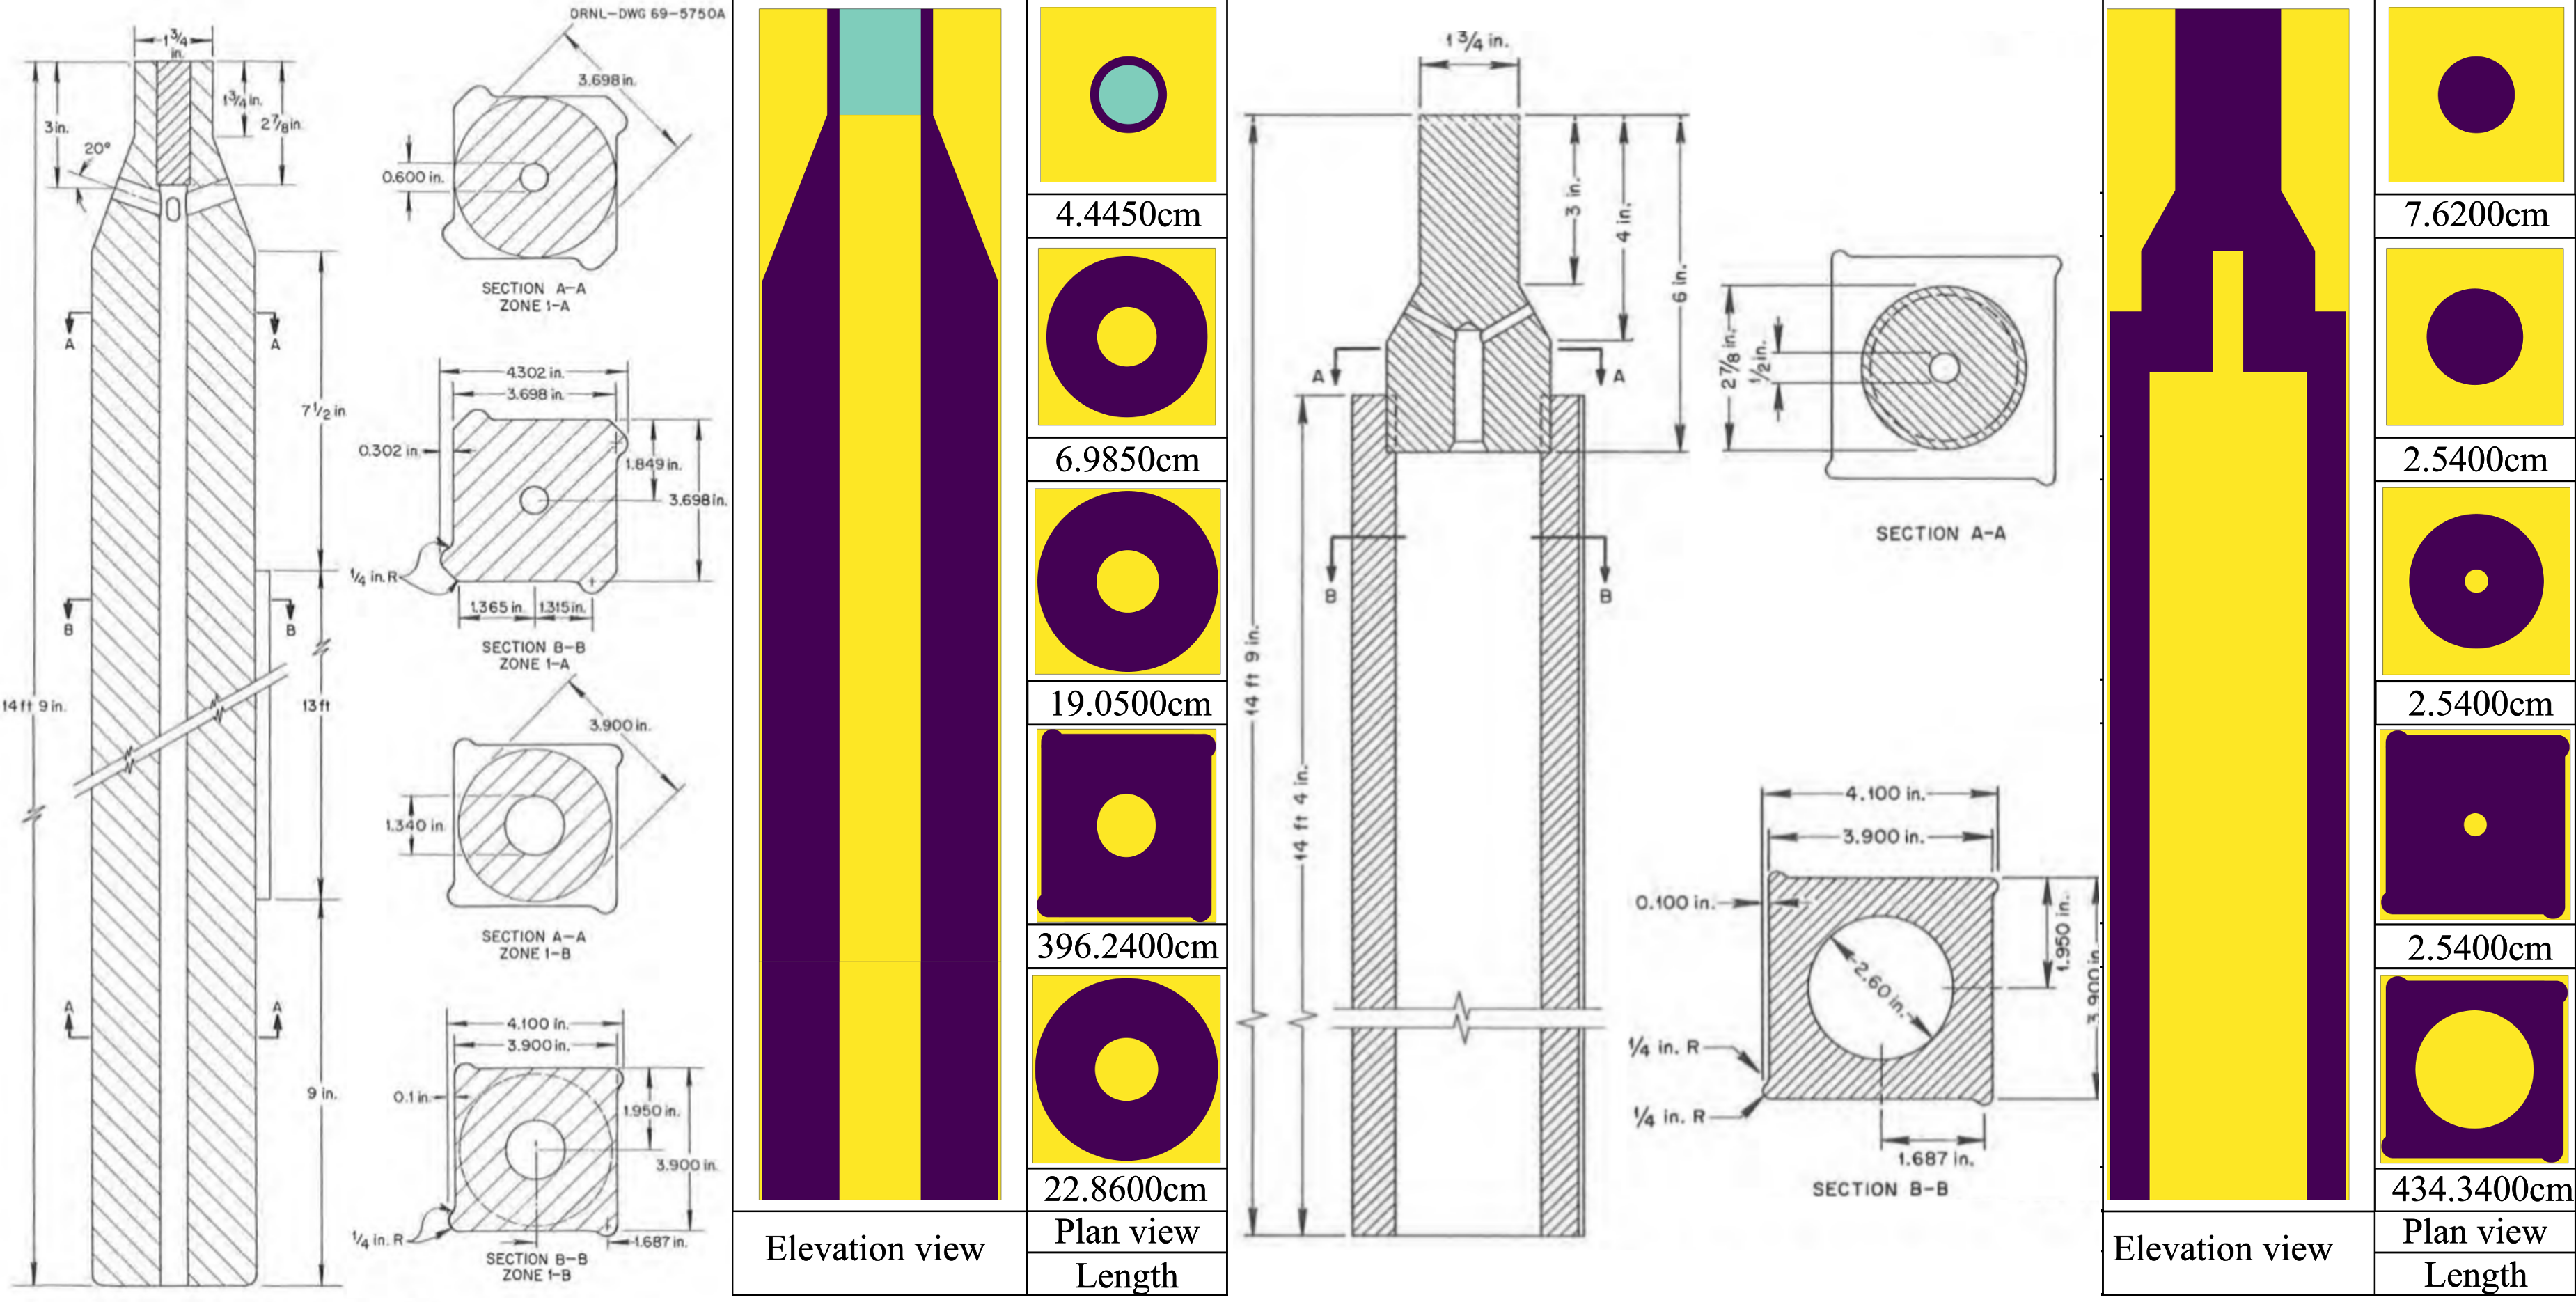
\includegraphics[height=0.77\textheight]{./images/zone_I_element.png}
            \vspace{-0.05in}
            \caption{Zone I (left) and Zone II (right) reference design
              \cite{robertson_conceptual_1971} and model.}
  \end{figure}
  
           \vspace{-0.1in}
      Volume fraction of fuel salt in zones I and II was 0.132 and 0.37 respectively.
     
\end{frame}

\begin{frame}
  \frametitle{Core Zone II}
  \begin{figure}[t]
     \vspace{-0.25in}
       \hspace*{-0.43in}
       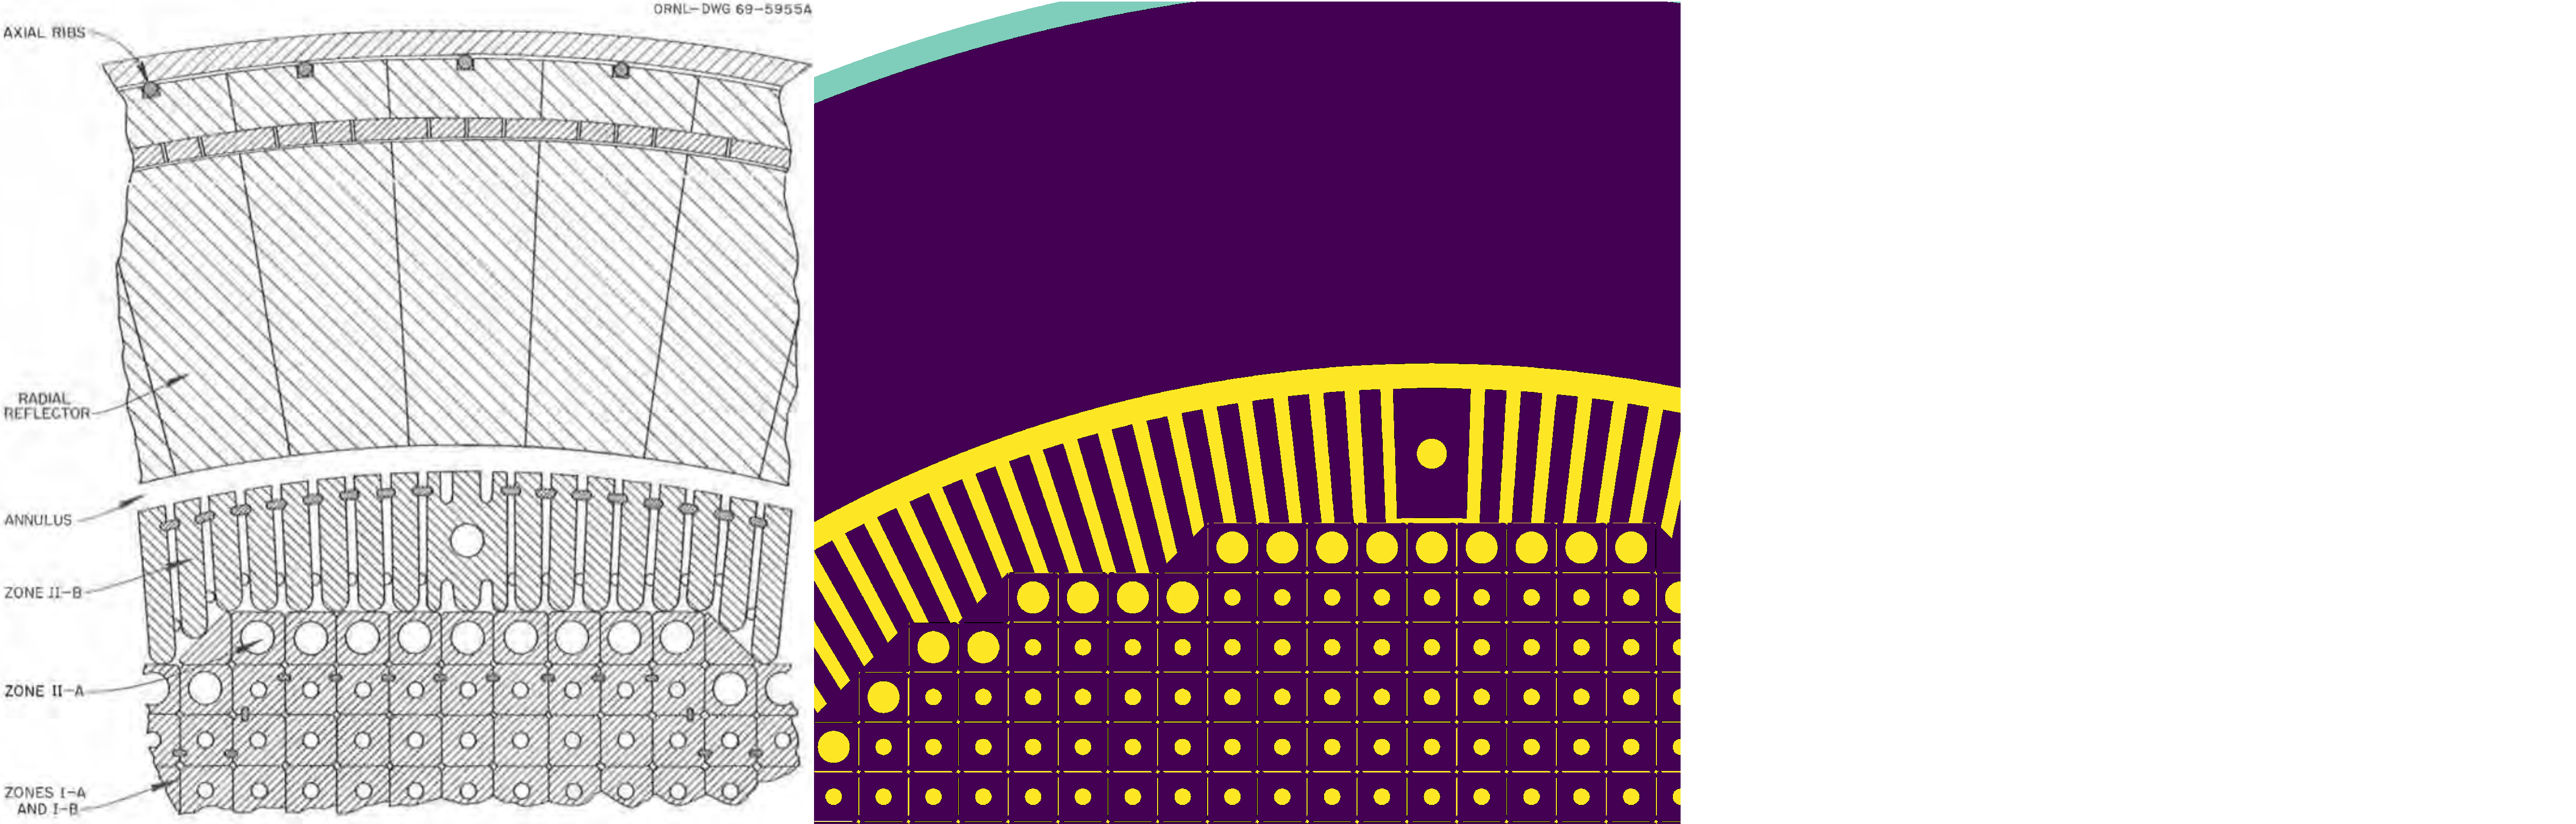
\includegraphics[height=0.77\textheight]{./images/reflector_and_elements.png}
            \caption{Detailed plan view of graphite reflector and moderator elements.}
  \end{figure}
           \vspace{-0.1in}
\end{frame}

\begin{frame}
  \frametitle{Approximations and assumptions}
              \begin{block}{Geometry simplifications}
               \begin{enumerate}
               \item Zone II-B elements simplified into right-circular
                 cylindrical shapes with central channels.
               \item Axial ribs in Zone I outer layer, Zone II-B and reflector was not
                 described in the model.
               \end{enumerate}
               \end{block}

               \begin{block}{Simulation conditions and nuclear data}
               \begin{enumerate}
               \item Two graphite control rods are fully inserted.
               \item Two safety rods are fully withdrawn.
               \item Moderator and fuel temperature is 900K.
               \item $10^5$ neutrons per cycle for a total of 1000 cycles,
                 the first 50 are inactive.
               \item ENDF/B-VII cross sections were used.
               \end{enumerate}
               \end{block}
\end{frame}

